\section{Auswertung}

\subsection{Gaußsche Fehlerfortpflanzung}

Wenn zu Messdaten die Standardabweichung bekannt ist, und mit diesen Messdaten weiter gerechnet werden soll,
wird die Gaußsche Fehlerfortpflanzung verwendet. 
Angenommen, es gibt $k$ Messwerte $x_i [i \in \mathbb{N}, i \leq k]$ mit den Standardabweichungen $\Delta x_i$
und eine abgeleitete Größe $f(x_i)$.
Dann ist der Fehler von $f$
\begin{align}
    \Delta f(x_i) = \sqrt{
    \left(\frac{\partial f}{\partial x_1} \Delta x_1\right)^2%
     + \left(\frac{\partial f}{\partial x_2} \Delta x_2\right)^2%
     + \dots%
     + \left(\frac{\partial f}{\partial x_k} \Delta x_k\right)^2%
    }.
    \label{eq:gauspflanz}
\end{align} 
Im Ergebnis ergibt sich der Mittelwert von $f$ mit der errechneten Abweichung $\overline{f} \pm \Delta f $.
Um Rechenfehler zu vermeiden, wird das Python \cite[]{python} Paket \texttt{uncertainties} \cite[][]{uncertainties} verwendet.
Hier wird die Fehlerfortpflanzung automatisch verrechnet, wenn die Variablen als \texttt{ufloat} definiert werden.




\subsection{Untersuchung des Geiger-Müller-Bereichs}

Die Impulsrate $N$ und die Stormstärke $I$ in Abhängigkeit der Spannung $U$ sind in Tabelle \ref{tab:impulsrate} zu sehen.
Der Fehler auf die Impulsrate errechnet sich dabei für jeden Wert gemäß $\sqrt{N}$. % und ergibt für jeden Wert \qty[]{1}{\per\second},
% was einer maximalen Prozentualen Abweichung von \num[]{0.89} \, \% entspricht.
Für die Messungenauigkeit von $I$ wird ein Ablesefehler von \qty[]{0.05}{\micro\ampere} geschätzt.


\begin{table}[H]
    \centering
    \caption{Die Impulsrate $N$ pro Sekunde und die Stromstärke $I$ in Abhängigkeit der Spannung $U$.}
    \label{tab:impulsrate}
    \begin{tabular}{
        S[table-format = 3.0] %U
        S[table-format = 3.0] @{${}\pm{}$} S[table-format = 1.0] %N
        S[table-format = 1.1] %I
        }
        \toprule
        {$U / \unit{\volt}$} & \multicolumn{2}{c}{$N / (\unit{\per\second})$} & {$I / \unit{\micro\ampere}$} \\
        \midrule
        310 & 104 & 10 & 0.1 \\
        330 & 192 & 14 & 0.2 \\
        350 & 192 & 14 & 0.2 \\
        370 & 195 & 14 & 0.2 \\
        390 & 195 & 14 & 0.3 \\
        410 & 197 & 14 & 0.4 \\
        430 & 198 & 14 & 0.4 \\
        450 & 201 & 14 & 0.5 \\
        470 & 200 & 14 & 0.5 \\
        490 & 198 & 14 & 0.6 \\
        510 & 199 & 14 & 0.6 \\
        530 & 199 & 14 & 0.7 \\
        550 & 199 & 14 & 0.7 \\
        570 & 201 & 14 & 0.8 \\
        590 & 201 & 14 & 0.8 \\
        610 & 203 & 14 & 0.9 \\
        630 & 204 & 14 & 1.0 \\
        650 & 208 & 14 & 1.0 \\
        670 & 209 & 14 & 1.1 \\
        690 & 213 & 15 & 1.1 \\
        710 & 218 & 15 & 1.2 \\
        730 & 222 & 15 & 1.2 \\
        \bottomrule       
    \end{tabular}
\end{table}



\subsubsection[]{Die Impulsrate}
Wird $N$ in Abhängigkeit von $U$ geplottet, ergibt sich Abbildung \ref{fig:impulsrate}.
Das Plateau wird auf den Spannungbereich \qtyrange[]{330}{630}{\volt} eingegrenzt und anschließend eine lineare Ausgleichsrechnung
\begin{align}
    N = s_\text{P} \cdot U + b 
\end{align}
mit Hilfe der Python \cite[]{python} Funktion \texttt{curve\_fit} aus dem Paket \texttt{scipy} \cite[]{scipy} durchgeführt.
Es ergeben sich die Werte 
\begin{align}
    s_\text{P} &= (0.032 \pm 0.004) \, \unit{\per\volt\per\second}, & b &= (182.770 \pm 1.998) \, \unit{\per\second}.
\end{align}
Die Ausgleichsgerade im Plateaubereich ist ebenfalls in Abbildung \ref{fig:impulsrate} zu sehen.
Der Arbeitspunkt des Zählrohrs kann somit ca. zu \qty[]{450}{\volt} bestimmt werden und die durchschnittliche Rate beträgt 
\qty[]{198 +- 4}{\per\second} im Plateaubereich.

\begin{figure}[H]
    \centering
    \includegraphics[height = 8.5cm]{build/teil1_rate.pdf}
    \caption{Die Impulsrate $N$ in Abhängigkeit der Spannung $U$.}
    \label{fig:impulsrate}
\end{figure}



\subsubsection[]{Die Ladungsanzahl}
Anhand der Stromstärke $I$ aus Tabelle \refeq{tab:impulsrate} wird die Ladungsträgeranzahl $Z$ gemäß
\begin{align}
    Z = \frac{I T}{e_0}
\end{align}
mit der Intervallzeit $T = \qty[]{120}{\second}$ und der Elementarladung $e_0$ berechnet.
Anschließend wird $Z$ in Abhängigkeit der Spannung geplottet (vgl. Abbildung \ref{fig:ladungszahl}) und erneut eine lineare Ausgleichsrechnung
\begin{align}
    Z = m \cdot U + n
    \label{eq:ladungszahl}
\end{align}
durchgeführt.
Es ergeben sich dabei die Parameter
\begin{align}
    m &= (2010 \pm 39) \cdot 10^9 \, \unit{\per\volt\per\second},  & n = (-552 \pm 21) \cdot 10^{12} \, \unit{\per\second}.
\end{align}
Damit die beiden berechneten Steigungen verglichen werden können, muss die Steigung der Ladungsanzahl gemäß \eqref{eq:ladungszahl}
zurücktransformiert werden.
Mit der Intervallnummer $x$ ergibt sich dabei die Steigung
\begin{align}
    \tilde{s}_\text{L} = \frac{e_0 x}{I T} \cdot m,
\end{align}
für jedes Intervall.
Hiervon werden Mittelwert und Standardabweichung berechnet, sodass sich schließlich die Steigung 
$s_\text{L} = (0.045 \pm 0.001) \, \unit{\per\volt\per\second}$ ergibt.
Die beiden Steigungen haben also eine Abweichung von $|s_\text{P} - s_\text{L}|/s_\text{L} = (28 \pm 10) \, \%$ zu einander.

\begin{figure}[H]
    \centering
    \includegraphics[height = 8.5cm]{build/teil1_ladungszahl.pdf}
    \caption{Die Impulsrate $N$ in Abhängigkeit der Spannung $U$.}
    \label{fig:ladungszahl}
\end{figure}






\subsection[]{Die Totzeit}

\subsubsection[]{Ablesen am Oszilloskop}
In Abbildung \ref{fig:totzeit_oszi} ist ein Foto des Bildes am Oszilloskop zu sehen.
Durch Ablesen des Abstandes zwischen Extremstelle und darauf folgender Nullstelle (vgl. Abbildung \textbf{REF!!! BILD ZUR TOTZEIT AUS THEORIE}) ergibt 
sich eine Totzeit von $\tau_\text{oszi} = \qty[]{95 +- 7}{\micro\second}$.
% ABLESEN AM OSZI:
% totzeit_oszi (9.5+/-0.7)e-05 μs

\begin{figure}[H]
    \centering
    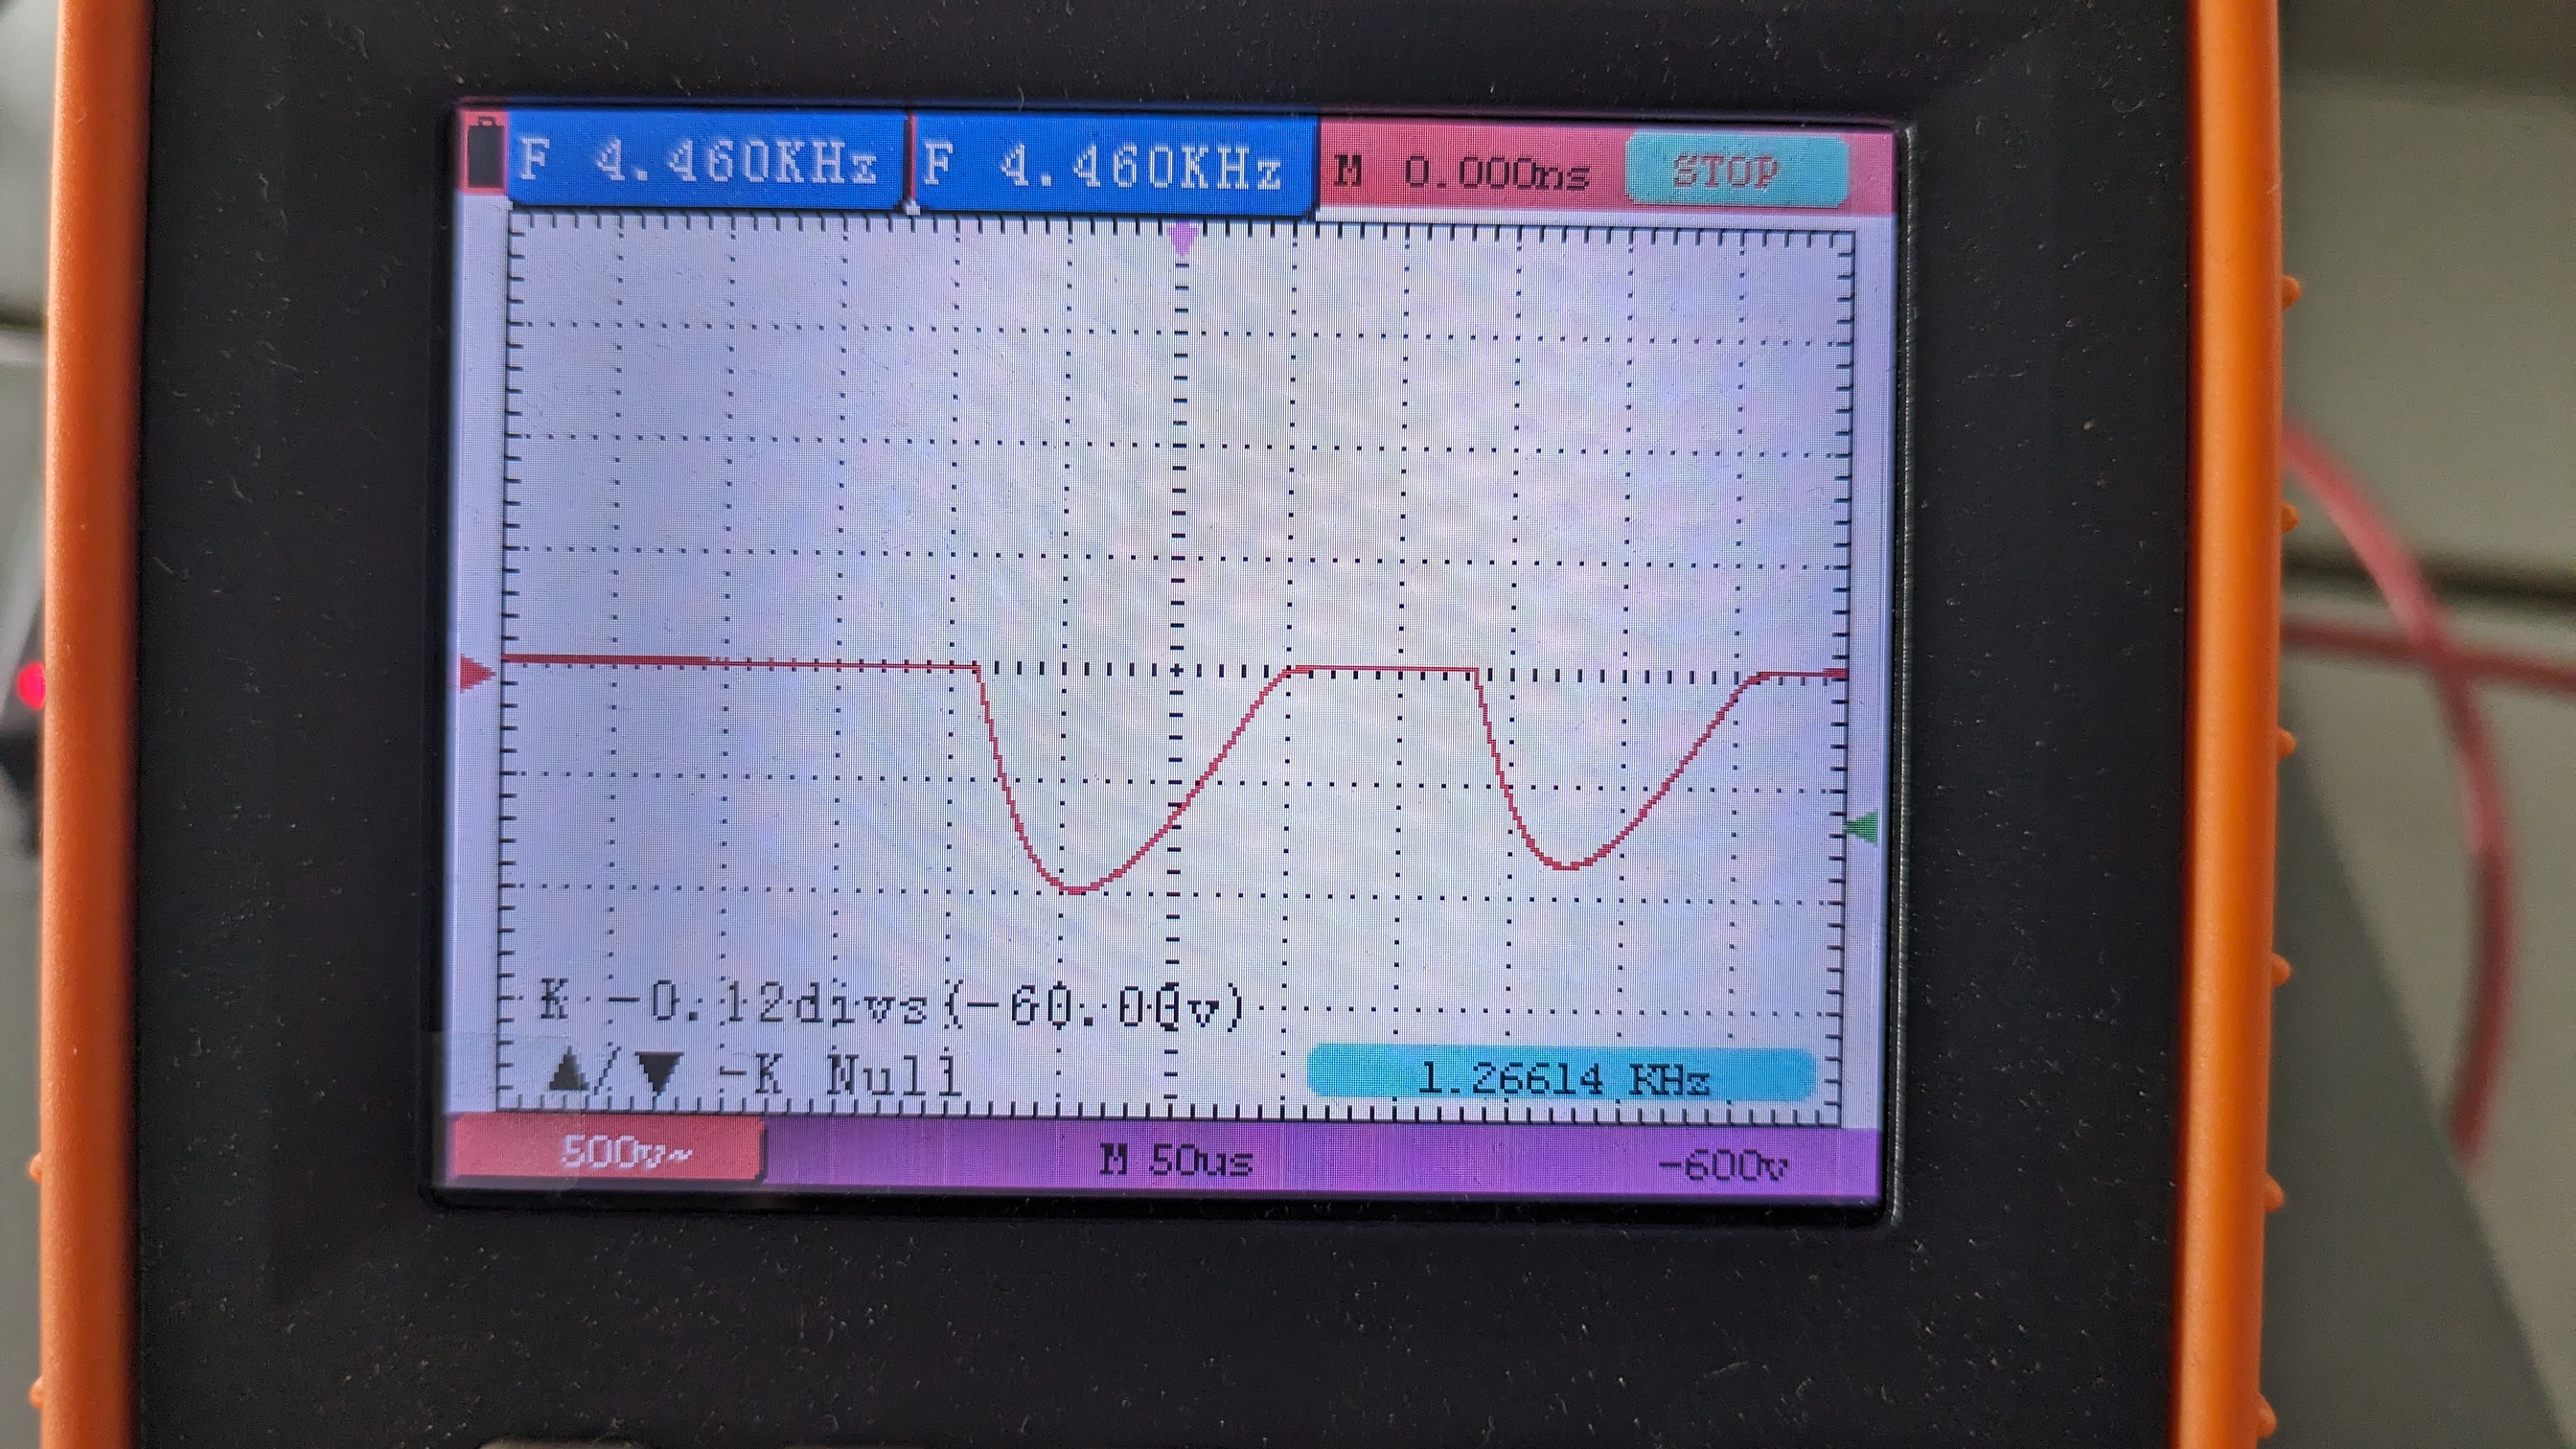
\includegraphics[height = 7.5cm]{Abbildungen/totzeit.jpg}
    \caption{Die Anzeige des Oszilloskops zur Bestimmung der Totzeit.}
    \label{fig:totzeit_oszi}
\end{figure}

\subsubsection[]{Berechnung nach der Zwei-Quellen-Methode}
Für die Zwei-Quellen-Methode werden die folgenden Werte berechnet
\begin{align*}
    N_1 &= (1380 \pm 40) \, \unit{\per\second}, &
    N_2 &=  (880 \pm 30) \, \unit{\per\second}, \\
    N_{12} &= (2070 \pm 50) \, \unit{\per\second}.
\end{align*}
Dabei wurde erneut durch die jeweilige Intervallzeit $T$ geteilt.
Die Fehler berechnen sich wie zuvor aus der Wurzel der Messwerte.

\noindent
Gemäß Gleichung \textbf{REF!!! TOTZEIT FORMEL} errechnet sich die Totzeit $\tau_\text{calc} = \qty[]{120 +- 60}{\micro\second}$.
Dies entspricht einer Abweichung von $(\tau_\text{oszi} - \tau_\text{calc}) / \tau_\text{calc} = (\num[]{20+-40})$ \, \%.

% ZWEI QUELLEN METHODE:
% n1:  (1.38+/-0.04)e+03
% n2:  880+/-30
% n12:  (2.07+/-0.05)e+03
% totzeit_calc 0.00012+/-0.00006
% Abweichung:  -0.2+/-0.4